\documentclass[a4paper, 12pt]{ctexart}
\setlength{\parindent}{2em}
\usepackage[
  a4paper,
  scale=0.78
]{geometry}
\usepackage{titlesec}
\usepackage{amsmath}
\usepackage{amssymb}
\usepackage{array}
\usepackage{booktabs}
\usepackage{graphicx}
\usepackage{float}
\usepackage[labelsep=period]{caption}
\usepackage{fvextra}
\usepackage{fancyhdr}
\usepackage{tabularx}
\usepackage[colorlinks=true, linkcolor=black, urlcolor=blue]{hyperref}

\setlength{\tabcolsep}{12pt} % 调大列间距
\graphicspath{{figures/hw11}}
\newcommand{\sat}{\operatorname{sat}}

% 调整标题格式，使其适合常规课程报告.
\titleformat{\section}
  {\normalfont\bfseries\Large}
  {\thesection}{0.8em}{}
\titlespacing{\section}{0pt}{18pt}{8pt}

\titleformat{\subsection}
  {\normalfont\bfseries\large}
  {\thesubsection}{0.8em}{}
\titlespacing{\subsection}{0pt}{12pt}{6pt}

% 设置源码附录的统一外观.
\fvset{
  fontsize=\scriptsize,
  frame=single,
  numbers=left,
  numbersep=6pt,
  breaklines=true,
  tabsize=4
}


% 设置页眉页脚：页眉留空，页脚居中显示页码.
\pagestyle{fancy}
\fancyhf{}
\cfoot{{\footnotesize\thepage}}
\renewcommand{\headrulewidth}{0pt}
\renewcommand{\footrulewidth}{0pt}
\fancypagestyle{plain}{
  \fancyhf{}
  \cfoot{{\footnotesize\thepage}}
  \renewcommand{\headrulewidth}{0pt}
  \renewcommand{\footrulewidth}{0pt}
}

\begin{document}

\begin{center}
  {\zihao{3}\bfseries 直流电机控制仿真}
\end{center}

\vspace{1em}

\tableofcontents
\clearpage

\section{电机参数与数学模型}

\subsection{电机参数}

本报告选用题目给出的 \textbf{RE 40 150W} 电机参数. 为便于数值仿真，将参数统一换算到 SI 制如下.

\begin{table}[H]
  \centering
  \caption{RE 40 150W 电机参数}

  \begin{tabular}{clc}
    \toprule
    参数           & 数值                                     & 单位                     \\
    \midrule
    电阻 $R$       & $24.4$                                 & $\Omega$               \\
    电感 $L$       & $6.41\times10^{-3}$                    & $\mathrm{H}$           \\
    力矩常数 $K_t$   & $0.266$                                & $\mathrm{N\cdot m/A}$  \\
    反电动势常数 $K_e$ & $\dfrac{1}{35.9}\cdot\dfrac{60}{2\pi}$ & $\mathrm{V/(rad/s)}$   \\
    转子惯量 $J$     & $1.2\times10^{-5}$                     & $\mathrm{kg\cdot m^2}$ \\
    供电电压上限 $U$   & $48$                                   & $\mathrm{V}$           \\
    \bottomrule
  \end{tabular}
\end{table}

\subsection{电机状态方程}

取状态量为
\[
  \boldsymbol{x} =
  \begin{bmatrix}
    \theta & \omega & i
  \end{bmatrix}^{\mathrm{T}},
\]
其中 $\theta$ 为转子位置，$\omega=\frac{\mathrm{d}\theta}{\mathrm{d}t}$ 为转速，$i$ 为电枢电流.

电机方程由电气部分和机械部分组成，分别为
\[
  u = L\frac{\mathrm{d}i}{\mathrm{d}t} + Ri + K_e \omega,
\]
\[
  J_{\text{total}}\frac{\mathrm{d}\omega}{\mathrm{d}t} = K_t i - \tau_L,
\]
其中 $u$ 为电压输入，$J_{\text{total}}$ 为总转动惯量，$\tau_L$ 为负载力矩.


\subsection{摩擦模型}

考虑黏性摩擦与库仑摩擦，摩擦模型写为
\[
  \tau_L
  =
  B\omega +
  \tau_c \tanh\!\left(\frac{\omega}{\omega_s}\right),
\]
其中：$B\omega$ 表示与速度成正比的黏性摩擦，$\tau_c$ 表示库仑摩擦幅值，$\tanh(\omega/\omega_s)$ 用于平滑符号函数.

\section{控制器设计}

\subsection{开环控制}

开环算例中直接向电机施加 $48\,\mathrm{V}$ 阶跃电压，不使用反馈调节. 其目的在于观察不同负载条件下，电机转速与电流随时间的变化规律.

\subsection{电流环控制}

电流环采用 PI 控制：
\[
  u = \sat\!\left(K_{pi}(i_r - i) + K_{ii}\int (i_r - i)\,\mathrm{d}t,\; U_{\mathrm{lim}}\right)
\]
其中 $\sat(x, x_{\mathrm{lim}})=\min(\max(x,-x_{\mathrm{lim}}),x_{\mathrm{lim}})$ 表示对称限幅函数，$U_{\mathrm{lim}}$ 为电压限幅值.

\subsection{速度环控制}

速度环采用串级结构. 外层速度 PI 先生成电流参考：
\[
  i_r = \sat\!\left(K_{p\omega}(\omega_r-\omega) + K_{i\omega}\int(\omega_r-\omega)\,\mathrm{d}t,\; i_{\mathrm{lim}}\right)
\]
由电流环跟踪该电流参考，最终输出电压指令，其中电流参考限幅用于避免过大的瞬时驱动力矩.

\subsection{位置环控制}

位置环采用位置 P + 速度 PI + 电流 PI 的三级串级结构. 最外层根据位置误差生成速度参考：
\[
  \omega_r = \sat\!\left(K_{p\theta}(\theta_r-\theta),\; \omega_{\mathrm{lim}}\right)
\]
随后依次由速度环与电流环进行控制，其中速度参考限幅用于约束位置误差较大时的指令峰值.

\section{仿真结果与分析}

\subsection{不同负载下的开环响应}

\begin{figure}[H]
  \centering
  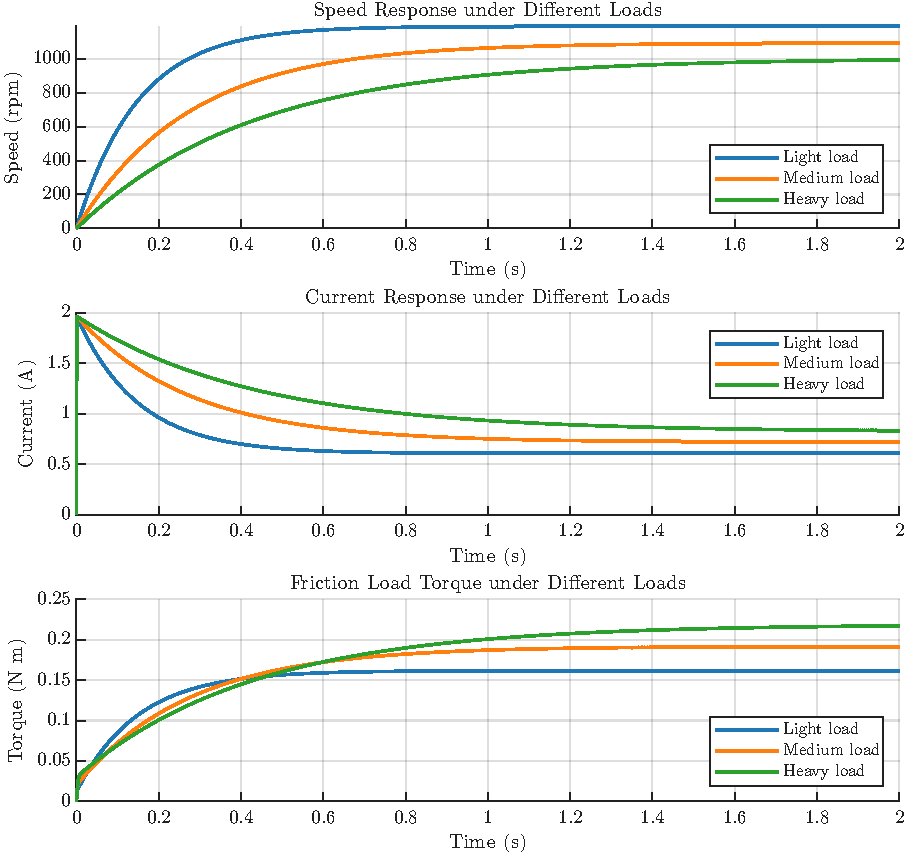
\includegraphics[width=0.88\textwidth]{Open Loop Responses.pdf}
  \caption{不同负载下的开环响应曲线}
\end{figure}

开环仿真对轻载、中载和重载三种不同的负载条件进行了仿真，三者的负载惯量、库仑摩擦幅值与黏性摩擦系数均递增. 上图展示了在这三种负载条件下电机的阶跃响应，可以观察到：
\begin{itemize}
  \item 负载惯量越大，电机加速响应过程越慢；
  \item 摩擦负载力矩越大，稳态电流越高，稳态转速越低.
\end{itemize}

\subsection{电流环控制结果}

\begin{figure}[H]
  \centering
  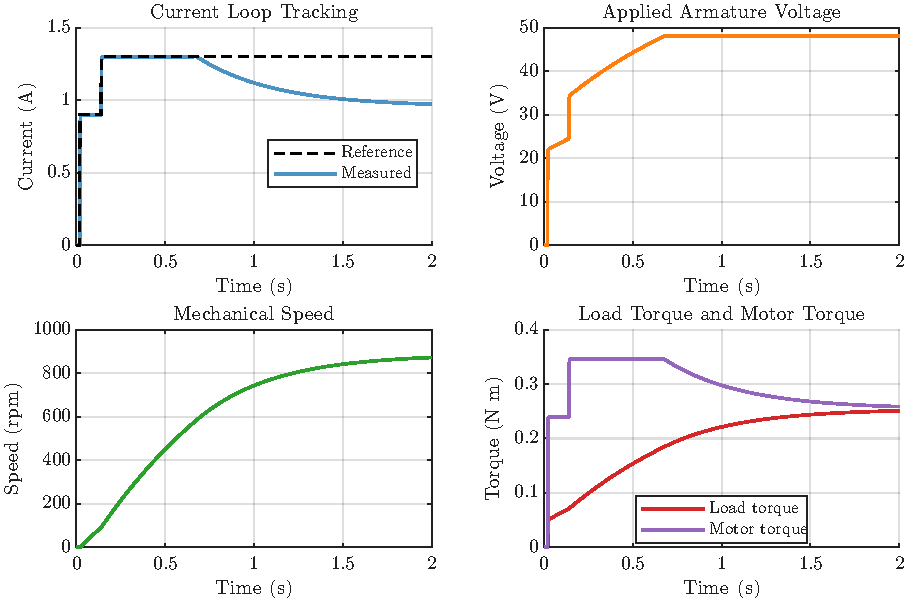
\includegraphics[width=0.88\textwidth]{Current Loop Control.pdf}
  \caption{电流环控制响应曲线}
\end{figure}

电流环控制算例跟踪一个两次阶跃的电流指令，响应曲线如上图所示，可以观察到：
\begin{itemize}
  \item 实际电流能够在指令改变后快速跟踪，几乎没有响应延迟；
  \item 由于缺乏足够的摩擦负载，转速会在常值电流驱动下持续上升，直至电压达到上限；
  \item 电压达到上限后，电流降低偏离指令，最终使得驱动力矩与摩擦力矩达到平衡.
\end{itemize}

\subsection{速度环控制结果}

\begin{figure}[H]
  \centering
  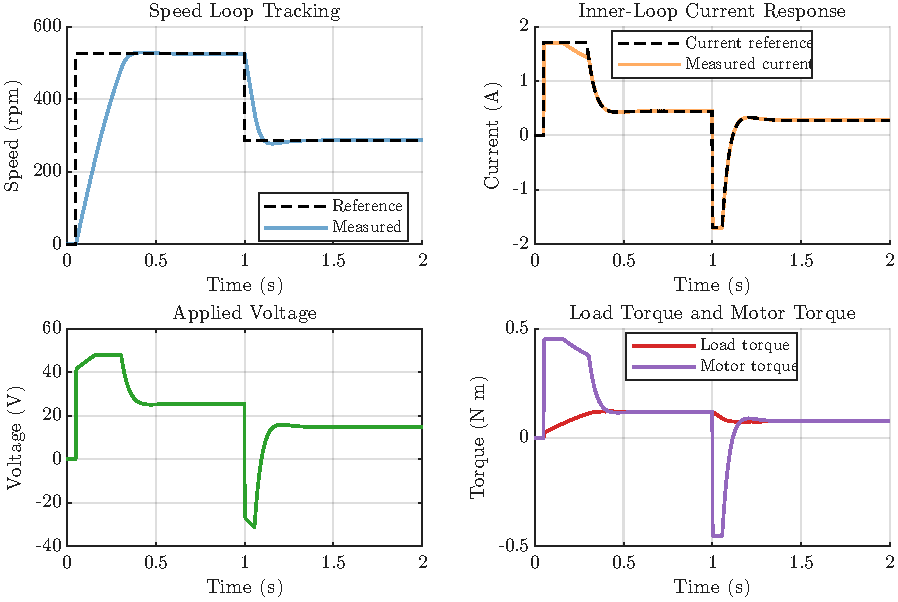
\includegraphics[width=0.88\textwidth]{Speed Loop Control.pdf}
  \caption{速度环控制响应曲线}
\end{figure}

速度环控制算例跟踪一个两次阶跃的速度指令，响应曲线如上图所示，可以观察到：
\begin{itemize}
  \item 实际转速能够较快地跟踪参考转速，迅速收敛到稳态；
  \item 电流参考在加速和减速瞬间分别给出较大的正、负峰值，实际电流基本能够紧跟参考变化；
  \item 力矩曲线表明：加速时驱动力矩明显大于摩擦负载力矩以完成加速，而在稳态阶段二者逐渐接近平衡；减速阶段驱动力矩短时变为负值，从而实现主动制动并建立新的速度平衡.
\end{itemize}

\subsection{位置环控制结果}

\begin{figure}[H]
  \centering
  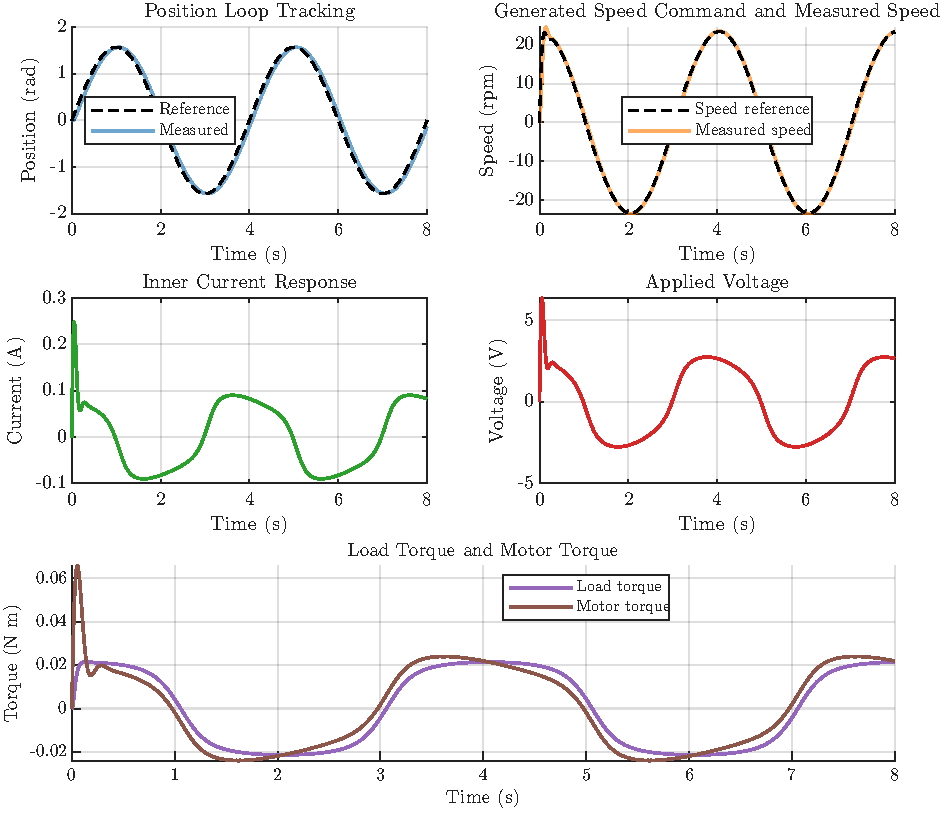
\includegraphics[width=0.88\textwidth]{Position Loop Control.pdf}
  \caption{位置环控制响应曲线}
\end{figure}

位置环控制算例跟踪一个正弦位置指令，响应曲线如上图所示，可以观察到：
\begin{itemize}
  \item 实际位置能够较好地跟踪正弦参考，整体波形与参考基本一致，仅存在较小的相位滞后和幅值误差；
  \item 力矩图表明驱动力矩与摩擦负载力矩整体呈现一个有相位差的周期性曲线，从而驱动电机周期性变速；
  \item 在起始阶段驱动力矩有一个短时峰值，以提供额外转矩完成从静止开始的快速加速.
\end{itemize}

\appendix
\clearpage
\section{代码文件组织}

本次作业的 MATLAB 程序位于 \texttt{MATLAB\_workspace/hw11\_motor/}， 各文件功能整理如下表所示.

\begin{table}[H]
  \centering
  \caption{代码文件组织说明}
  \begin{tabular}{ccc}
    \toprule
    文件                                      & 类型   & 作用说明           \\
    \midrule
    \nolinkurl{motor_open_loop.m}           & 入口脚本 & 完成开环电压驱动下的仿真   \\
    \nolinkurl{motor_current_loop.m}        & 入口脚本 & 完成电流环控制仿真      \\
    \nolinkurl{motor_speed_loop.m}          & 入口脚本 & 完成速度环控制仿真      \\
    \nolinkurl{motor_position_loop.m}       & 入口脚本 & 完成位置环控制仿真      \\
    \nolinkurl{getMotorParams.m}            & 共享函数 & 统一管理电机参数       \\
    \nolinkurl{simulateMotorResponse.m}     & 共享函数 & 统一实现电机数值仿真     \\
    \nolinkurl{+utils/createFigureA4.m}     & 辅助函数 & 创建统一尺寸的图窗      \\
    \nolinkurl{+utils/setDefaultGraphics.m} & 辅助函数 & 设置默认图形属性       \\
    \nolinkurl{+utils/tab10Color.m}         & 辅助函数 & 返回 Tab10 调色盘颜色 \\
    \bottomrule
  \end{tabular}
\end{table}

\section{MATLAB 源码}

\subsection*{\texttt{motor\_open\_loop.m}}
\VerbatimInput{../MATLAB_workspace/hw11_motor/motor_open_loop.m}

\subsection*{\texttt{motor\_current\_loop.m}}
\VerbatimInput{../MATLAB_workspace/hw11_motor/motor_current_loop.m}

\subsection*{\texttt{motor\_speed\_loop.m}}
\VerbatimInput{../MATLAB_workspace/hw11_motor/motor_speed_loop.m}

\subsection*{\texttt{motor\_position\_loop.m}}
\VerbatimInput{../MATLAB_workspace/hw11_motor/motor_position_loop.m}

\subsection*{\texttt{getMotorParams.m}}
\VerbatimInput{../MATLAB_workspace/hw11_motor/getMotorParams.m}

\subsection*{\texttt{simulateMotorResponse.m}}
\VerbatimInput{../MATLAB_workspace/hw11_motor/simulateMotorResponse.m}

\subsection*{\texttt{+utils/createFigureA4.m}}
\VerbatimInput{../MATLAB_workspace/+utils/createFigureA4.m}

\subsection*{\texttt{+utils/setDefaultGraphics.m}}
\VerbatimInput{../MATLAB_workspace/+utils/setDefaultGraphics.m}

\subsection*{\texttt{+utils/tab10Color.m}}
\VerbatimInput{../MATLAB_workspace/+utils/tab10Color.m}

\end{document}
